	Pour ce projet, nous avons décider d'installer Windows Server 2003 Entreprise Edition, afin d'avoir un sytème d'exploitation récent. Toutes les fonctionnalités utilisées pour la création d'un VPN sont incluses dans cette version. Il n'y a pas besoin d'installer une application tierce.
	Voyons à présent les différents services nécessaires pour la mise en place du VPN de Microsoft.

\subsubsection{Services installés}

	Afin de pouvoir se mettre dans les conditions du réseau interne de l'ISIMA, nous avons décidé de configurer plusieurs services:
~


\begin{itemize}
	\item  DHCP,
	\item  DNS, 
	\item  Active Directory,
	\item  Routage et accès distant (VPN),
	\item  Autorité de certification (CA).
\end{itemize}
~	

	Ces nombreux services sont nécessaires pour la création d'un VPN. A présent, détaillons la configuration de chacun de ces servives. 
	Remarque : Sous windows on ne parle pas de serveur mais de service. Tout les fonctionnalités de la machine (DNS, DHCP ou autre) sont référencés comme des services.


\paragraph{Caractéristique de la machine}
~\

Le serveur windows est installé sur un DELL PowerEdge 1300. Il est doté d'un processeur INTEL de type Pentium II cadencé à 348 Mhz. Il possède 512 Mo de mémoire vive et un disque dur de 9 Go.
Le serveur est composé de trois cartes réseaux, une pour le réseau extérieur et deux autres pour le réseau interne. 



Voici leur adresse IP:

\begin{figure}[H]
	\begin{center}
\begin{tabular}{|l|c|c|}
\hline
Caractéristique & Réseau & Adresse IP \\
\hline
Realtek RTL 8139 Familly & réseau PROFS & 10.0.0.11/24 \\
Realtek RTL 8139 Familly & réseau extérieur & 192.168.102.250/24 \\
Fast Ethernet CNET PRO 200P & réseau STUDENTS & 192.168.0.11/24 \\
\hline
\end{tabular}
	\end{center}
	\caption{Caractéristique des cartes réseaux}
	\label{IP_carte_reseau}
\end{figure}

Tout les cartes installés sont de type 100Mbit/s.
~

\paragraph{Service DHCP}
~\


Ce service est nécessaire pour l'attribution des adresses IP qui seront allouées aux différents clients lors de leurs connexion au serveur VPN. Nous avons configurer le service DHCP de la manière suivante. Sachant que le serveur VPN doit avoir deux cartes réseaux indépendantes (une sur le réseau STUDENTS et une sur le réseau PROFS) le DHCP peut fournir deux pools d'adresse différents. 
Voici les caractéristiques des deux réseaux:

\begin{figure}[H]
	\begin{center}
\begin{tabular}{|l|c|c|}
\hline
Caractéristique & Réseau PROFS & Réseau STUDENTS \\
\hline
Désignation Carte réseau & DHCP\_PROFS & DHCP\_STUDENTS \\
Adresse IP Carte réseau & 10.0.0.11 & 192.168.0.11 \\
Pool d'adresse & 10.0.2.100 à 10.0.2.254 & 192.168.0.100 à 192.168.0.254 \\
Masque réseau & 255.255.255.0 & 255.255.255.0 \\
Serveur DNS/routeur & 10.0.0.11 & 192.168.0.11 \\
Nom du domaine DNS & wvpn.isima.fr & wvpn.isima.fr \\
\hline
\end{tabular}
	\end{center}
	\caption{Caractéristique du service DHCP}
	\label{service_DHCP}
\end{figure}

Il est à noter que lors de l'installation du service DHCP, et en dehors des différentes configurations des cartes, il n'y a pas d'options spécifiques. Ce sont les options par défaut.
Il est à remarquer que le service DHCP se compose de deux étendues, une pour chaque carte. Cependant, le service DHCP s'attache à une seule carte réseau et non au deux. Dans la maquette, le service se lie avec la carte DHCP\_PROFS. Pour illustrer ces propos, voici un screenshot du service DHCP.

\begin{figure}[H]
	\begin{center}
	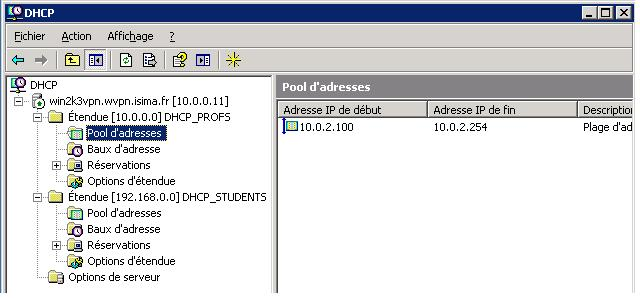
\includegraphics[width=\textwidth]{partie_2/screen_windows/dhcp.JPG}\\
	\end{center}
	\caption{Lien avec la carte réseau DHCP\_PROFS}
	\label{Screen_client_dhcp}
\end{figure}


On remarque que bien que la présence des deux étendues et que la carte DHCP\_PROFS (10.0.0.11) s'attache au service DHCP.
~\


Voyons à présent la configuration du service DNS.

\paragraph{Service DNS}
~\


Afin de pouvoir utiliser l'active directory nous avons du installer ce service. Celui-ci nous permet de résoudre les différentes adresses IP qui seront nécessaire lorsq'un client VPN se connectera sur le réseau interne.
Voici les caractèristiques du service DNS:
~\


\begin{figure}[H]
	\begin{center}
\begin{tabular}{|l|c|c|}
\hline
Caractéristique & Serveur Windows2003 \\
\hline
Nom de la machine &  win2k3vpn\\
Nom du domaine & wvpn.isima.fr\\
Type de zone &  zone principale\\
\hline
\end{tabular}
	\end{center}
	\caption{Caractéristique du service DNS}
	\label{service_DNS}
\end{figure}

~\

Il est à remarquer que lors de l'installation du service, nous avons décider d'incorporer la zone de recherche inversée. Le serveur windows étant composé de trois cartes réseaux, il y a trois zones. Afin de vérifier que le service DNS est bien configurer, la commande NSLOOKUP nous permet de tester le DNS. 
L'illustration suivante montre la résolution DNS est correcte.

\begin{figure}[H]
	\begin{center}
		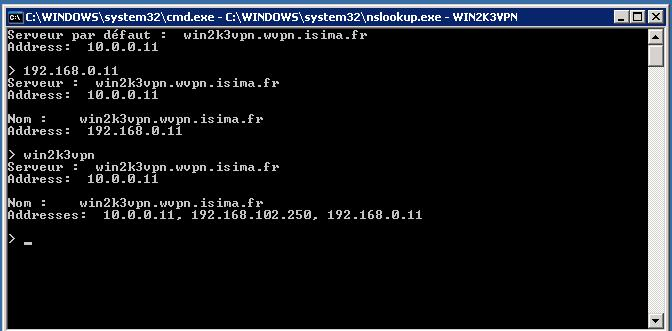
\includegraphics[width=\textwidth]{partie_2/screen_windows/nslookup.JPG}\\
	\end{center}
	\caption{Résolution DNS}
	\label{NSLOOKUP}
\end{figure}

Tout comme le service DHCP, le service DNS se lie avec une seule carte réseau. 

Intéressons nous à présent à la configuration de l'Active Directory.

\paragraph{Active Directory}
~\

Ce service nous a permi de créer un annuaire afin d'indentifier les clients souhaitant se connecter sur le réseau interne. Afin de pouvoir effectuer des tests sur la connexion VPN, nous avons dans un premier temps créeer deux groupes: un groupe STUDENTS et un groupe PROFS.

Il est à noter que lorsqu'on crée un utilisateur, on doit l'ajouter dans le groupe PROFS ou STUDENTS sans oublier de lui donner l'autorisation de pouvoir se connecter. 

\begin{figure}[H]
	\begin{center}
		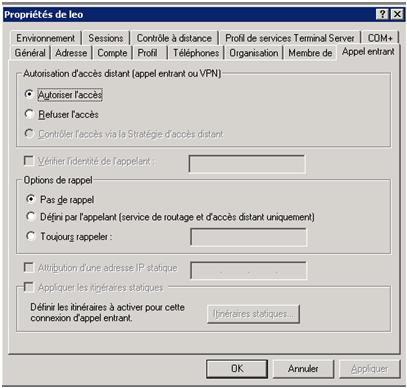
\includegraphics[width=0.50\textwidth]{partie_2/screen_windows/vpn.JPG}\\
	\end{center}
	\caption{Autorisation de se connecter via VPN sur le serveur Windows 2k3}
	\label{VPN_AUTORISATION}
\end{figure}

Du point de vue de la stratégie de groupe (GPO) nous avons décider de laisser la configuration par défaut.

Une fois les services de base installé, voyons à présent la configuration du service de \textit{Routage et accès distant} .

\paragraph{Routage et accès distant}
~\


Le service routage et accès distant est le service qui va nous permettre de monter un tunnel sécurisé. Lors de l'installation du service, l'administrateur doit choisir l'option ``routage pour réseaux locaux uniquement'' ainsi que l'option ``serveur d'accès distant''. Une fois le service installé, il faut configurer les options de sécurité qui sont propre au serveur (un clique droit sur le nom du serveur permet de modififer les propriétés). Cela correspond à la manière que les utilisateurs s'identifie. Le service propose deux choix : identification par l'annuaire ou bien en utilisant un serveur RADIUS.

\begin{figure}[H]
	\begin{center}
		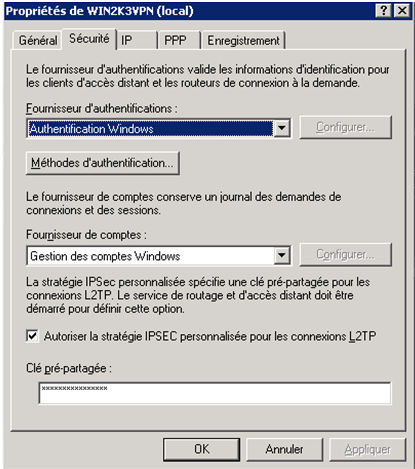
\includegraphics[width=0.50\textwidth]{partie_2/screen_windows/secu_vpn.PNG}\\
	\end{center}
	\caption{Choix de la méthode d'authentification}
	\label{VPN_AUTHENTIFICATION}
\end{figure}

Nous avons essayer de tester la maquette en utilisant le serveur RADIUS afin que celui-ci authentifie l'utilisateur avec la base NIS. Cependant les essais n'ont pas été concluant, nous n'avons pas pu nous identifier en utilisant notre compte ISIMA. Afin de rendre la maquette fonctionnel, nous avons dû laisser l'authentification par l'intermédiaire de l'annuaire local.

Dans l'onglet IP, il faut configurer la manière dont le service va distribuer les adresses IP. Ici nous avons le choix, soit le système gère les adresses IP en utilisant le service DHCP, soit l'administrateur peut remplir manuellement la plage d'adresse IP. La dernière option ``carte'' qui correpond à un menu déroulant nous permettant de selectionner la carte réseau qui repondrera aux demandes de la création d'un tunnel sécurisé. 

\begin{figure}[H]
	\begin{center}
		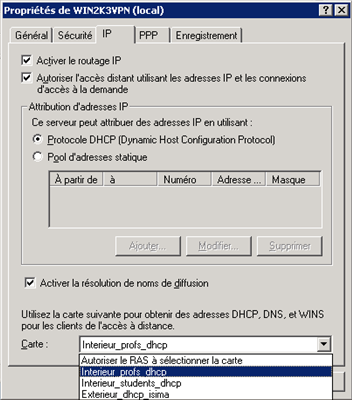
\includegraphics[width=0.50\textwidth]{partie_2/screen_windows/choix_carte.PNG}\\
	\end{center}
	\caption{Selection de l'interface réseau}
	\label{VPN_CARTE_ECOUTE}
\end{figure}

En naviguant dans les différentes options, on se rend rapidement compte que le service d'accès distant se lie avec une seule carte réseau. C'est la grande limitation. Il n'est pas possible que les deux cartes réseaux destinés pour le traffic interne redirige les différents flux réseaux.

D'un point de vue sécurité, il est possible de créer des stratégies d'accès distant. Pour le projet, nous avons créer une stratégie avec les spécifications suivantes:
~
\begin{itemize}
 	\item Appartenance à un groupe : PROFS ou STUDENTS
	\item Type d'authentification : MS-CHAP V2
	\item Spécification du type de connexion : VPN
\end{itemize}



Cette stratégie d'accès distant comporte une priorité de 1. Si un client respecte tous ces critères il pourra alors se connecter sur le serveur VPN.

\begin{figure}[H]
	\begin{center}
		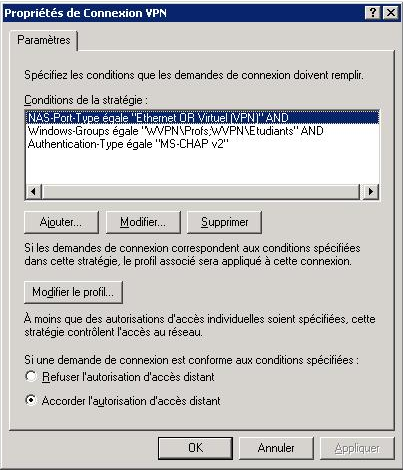
\includegraphics[width=0.50\textwidth]{partie_2/screen_windows/strat.png}\\
	\end{center}
	\caption{Stratégie d'accès distant}
	\label{VPN_STRAT}
\end{figure}

Dans la stratégie d'accès on peut rajouter un paramètre sur la date. En effet, on le paramétrant, on peut définir une plage horaire où l'utilisateur ne pourra pas se connecter.

Concernant le tyoe d'authentification, on utilise le protocole MS-CHAP V2 qui est un protocole propriétaire de Miscrosoft. En complement de cela, le serveur VPN fait un challenge de type MD5 afin d'authentifier le client.

Le protocole MS-CHAP V2 utilise une authentification mutuelle. Cela permet au serveur d'authentification et à la machine distante de vérifier leurs identités respectives. L'inconvenient de cette méthode d'authentification est que le login du client passe en clair sur le réseau. En sniffant la connexion par l'intermédiare de Wireshark, nous nous sommes rendu compte de cela. Par contre, le challenge MD5, et les mots de passe sont chiffrés.

